\documentclass[10pt]{beamer}
\usetheme{Madrid}
\usepackage[latin1]{inputenc}
\usepackage[spanish]{babel}
\usepackage{amsmath}
\usepackage{amsfonts}
\usepackage{amssymb}
\usepackage{graphicx}
\author{Daniel Remigio Valentin}
\title{Cadenas de Markov}
%\setbeamercovered{transparent} 
%\setbeamertemplate{navigation symbols}{} 
\logo{
\includegraphics[scale=0.3]{uni.jpg}} 
\institute{Universidad Nacional de Ingenier�a} 
\date{} 
%\subject{} 
\begin{document}

\begin{frame}
\titlepage
\end{frame}

%\begin{frame}
%\tableofcontents
%\end{frame}
%%%%%%%%%%%%%%%%Diapositiva 1 %%%%%%%%%%%%%%%%
\begin{frame}{Introducci�n}
	\textbf{\Large {Procesos Estoc�sticos :}} \newline 
	Una sucesi�n de de observaciones $ X_{1},X_{2},X_{3},\ldots,X_{n} $ se denomina \textbf{proceso estoc�stico} si verifica lo siguiente :
	\begin{itemize}
		\item Si los valores de estas observaciones no se pueden predecir exactamente. \pause
		\item Pero se pueden especificar las probabilidades para los distintos valores
posibles en cualquier instante de tiempo.\pause
	\end{itemize}
	Ahora tenemos que:\newline
	$ X_{1} $ : v.a. que define el \textbf{estado inicial del proceso}\newline
	$ X_{n} $ :  v.a. que define el \textbf{estado del proceso en el instante de tiempo} \emph{n}\newline \newline
	Para cada posible valor del estado inicial $s_1$ y para cada uno de los sucesivos valores
	$s_n$ de los estados $X_n, n=1,2,\ldots$ especificamos:
	\[P(X_{n+1}=s_{n+1})|X_1=s_1,X_2=s_2,\ldots,X_n=s_n\]
\end{frame}

%%%%%%%%%%%%%% Diapsitiva 2 %%%%%%%%%%%%%%
\begin{frame}{Cadenas de Markov}
\textbf{\Large {Propiedad Markoviana :}} \newline 
	Si el estado actual $ X_n $ y los estados previos $ X_1, \ldots, X_{n-1} $ son conocidos, entonces, la probabilidad del estado futuro $ x_{n+1} $, no depende de los estados anteriores $ X_1, \ldots , X_{n-1} $, y solamente depende del estado actual $X_n$, es decir para $n=1,2,\ldots$ y cualquier sucesi�n de estados $s_1,s_2,\ldots,s_{n+1}$\pause
	\[ P (X_{n+1} = s_{n+1} | X_1 = s_1, X_2 = s_2, . . . , X_n = s_n)= P (X_{n+1} = s_{n+1} | X_n = s_n) \]
\end{frame}

%%%%%%%%%%%%% Diapositiva 3 %%%%%%%%%%
\begin{frame}{Cadenas de Markov}{Cadenas de Markov finitas con probabilidades de transici�n estacionaria}
	
	\textbf{\large{Cadena de Markov finita}}\newline \newline
	Es una cadena de Markov para la que existe s�lo un n�mero finito k de
estados posibles $ s_1, \ldots , s_k $ y en cualquier instante de tiempo la cadena est�
en uno de estos k estados.\newline

	\textbf{\large{Probabilidad de transici�n}}\newline \newline
	Es la probabilidad condicionada:\pause \[P(X_{n+1}=s_{n+1}|x_n=s_n)\]
	
	\textbf{\large{Probabilidad de transici�n estacionaria}}\newline
	Una cadena de Markov tiene probabilidades de transici�n estacionarias
si para cualquier par de estados $s_i$ y $s_j$ existe una probabilidad de
transici�n pij tal que:\pause \[P (X_{n+1} = s_j | X_n = s_i) = pij \mbox{ para } n = 1, 2,\ldots\]
\end{frame}

%%%%%%%%%%%%% Diapositiva 4 %%%%%%%%%%
\begin{frame}{Cadenas de Markov}{Matriz Estoc�stica}
	Son aquellas matrices cuadradas cuyos elementos son no negativos y tal que la
suma de los elementos de cada fila es igual a 1. \newline \newline
	\textbf{\large{Matriz de transici�n en un solo paso}}\newline \pause
		$p_{ij} = P (X_{n+1} = s_j |X_n = s_i) \rightarrow P=\left(\begin{array}{lccc}

		p_{11} & p_{12} & \ldots & p_{1k} \\
		p_{21} & p_{22} & \ldots & p_{2k} \\
		\vdots & \vdots & \ddots & \vdots \\
		p_{k1} & p_{k2} & \ldots & p_{kk}
		\end{array} \right)$
		
	La matriz de transici�n P de cualquier cadena de Markov finita con
probabilidades de transici�n estacionarias es una matriz estoc�stica

	
\end{frame}

%%%%%%%%%%%% Diapositiva 5 %%%%%
\begin{frame}{Cadena de Markov}
\textbf{\large{Ejemplo}}: \newline \newline
	Supongamos que el clima de una determinada regi�n s�lo puede ser soleado
$ (s_1) $ o nublado $ (s_2) $ y que las condiciones del clima en ma�anas sucesivas forman
una cadena de Markov con probabilidades de transici�n estacionarias. La matriz
de transici�n est� dada por:\\ \pause
	\[ P=\left(\begin{array}{cc}
		0.7 & 0.3 \\
		0.6 & 0.4 \\
		\end{array} \right)\]

Si un d�a concreto est� nublado, cu�l es la probabilidad de que est� nublado
el d�a siguiente?.\[p_{22}=0.4\]
		
\end{frame}

%%%%%%%%%%%%%%%%%%%%%%%% Diapositiva 6 %%%%%%%%%%%%%%%%%%%%%%%%%%%
\begin{frame}{Cadenas de Markov}
\textbf{\large{Ejemplo}}: \newline \newline
 En un peque�o pueblo el clima puede cambiar, de un d�a para otro, consideremos 2 estados del tiempo: clima seco y clima h�medo. La probabilidad de tener un clima seco es 0.8, si el d�a actual es seco; pero si es h�medo la probabilidad de obtener un clima seco es de 0.6. Suponga que dichos valores no cambian en el tiempo. Se pide determinar:
 \begin{itemize}
 	\item Matriz de Transici�n.
 	\item Diagrama de transici�n.
 	\item La probabilidad de estado.
 \end{itemize}
 
 \textbf{Matriz de transici�n: \newline}
 X: Estado del clima 
 $X=\left\lbrace \begin{array}{ll}
 0 & \mbox{Clima seco} \\
 1 & \mbox{Clima h�medo} \\ 
 \end{array}\right.$

\end{frame}

%%%%%%%%%%%%%%%%%%% Diaposita 7 %%%%%%%%%%%%%%%%%%%%%%%%%%%%%%%%%%%%%
\begin{frame}{Cadenas de Markov}

La probabilidad de obtener un clima seco al d�a siguiente si hoy el clima esta seco:
 $P\left\lbrace X_{t+1}=0 | X_{t}=0\right\rbrace=0.8 $.  \\
La probabilidad de obtener un clima seco al d�a siguiente si hoy el clima esta h�medo:\\
 $P\left\lbrace X_{t+1}=0 | X_{t}=1\right\rbrace=0.6 $  \newline
luego tenemos: 
\\
 \begin{tabular}{|c|c|c|}
 \hline 
   & 0 & 1 \\ 
 \hline 
 0 & $ P_{00}=0.8$ & $P_{01}=0.2$  \\ 
 \hline 
 1 & $P_{10}=0.6$ & $P_{11}=0.4$ \\ 
 \hline 
 \end{tabular} 
 Donde $P_{ij}$:Probabilidad de pasar del clima i al clima j
\newline
Por lo tanto la matriz de transici�n es:\pause
$$M_{T}=\left(\begin{array}{cc}
0.8 & 0.2 \\
0.6 & 0.4 \\
\end{array} \right)$$

\textbf{Diagrama de transici�n}\pause
\begin{figure}
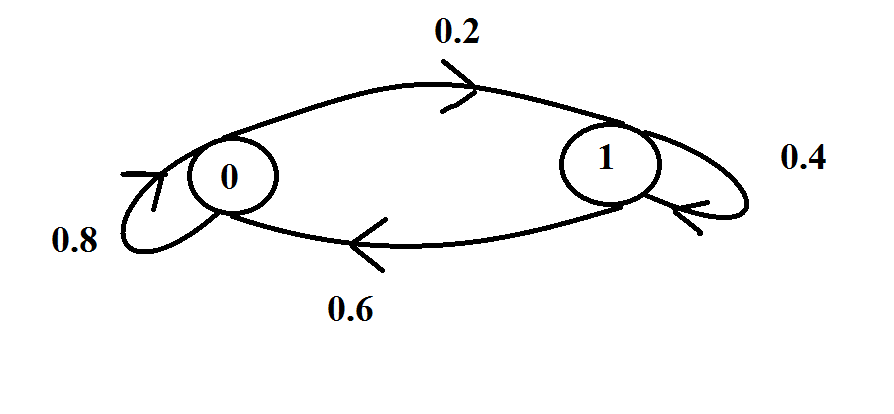
\includegraphics[scale=0.2]{diagrama_Markov.png}
\end{figure}

\end{frame}

%%%%%%%%%%%%%%%%%%%%%%%%%%% Diapositiva 8 %%%%%%%%%%%%%%%%5%%%
\begin{frame}{Cadenas de Markov}
\textbf{La probabilidad de estado estable del sistema}
\\

$\pi_{0}$:Probabilidad que cierto d�a sea seco
\\

$\pi_{1}$:Probabilidad que cierto d�a sea h�medo
\\
De lo anterior podemos concluir que :
\\
$ \pi_{0} + \pi_{1} =1 $
\\ entonces tenemos:
\\
$ \pi_{0} =1 - \pi_{1} $

\begin{eqnarray*}
\pi_{0} + \pi_{1} & = & 1 \\
\pi_{0}P_{00} + \pi_{1}P_{10} & = & \pi_{0} \\
\pi_{0}P_{01} + \pi_{1}P_{11} & = & \pi_{1}
\end{eqnarray*}
reemplazando tenemos que:\\\pause
$\pi_{0}=0.75$\\
$\pi_{1}=0.25$
\end{frame}

\end{document}